% Please use the skeleton file you have received in the
% invitation-to-submit email, where your data are already
% filled in. Otherwise please make sure you insert your
% data according to the instructions in PoSauthmanual.pdf
%\documentclass{PoS}
% \usepackage{enumitem}% http://ctan.org/pkg/enumitem
% \usepackage{cite}
% \usepackage{graphicx}
% \usepackage[toc,page]{appendix}
% \usepackage{url}
% \usepackage{hyperref}
% \usepackage[all]{hypcap} % Clicking puts you on top of figure

%\addcontentsline{toc}{chapter}{Scaling LOFAR Processing}                                                                                                     

\chapter[LOFAR Scalability Framework]{An Automated Scalable Framework for Distributing Radio Astronomy Processing Across Clusters and Clouds}\label{ch:GRID_LRT}


%\subtitle{Framework for distributing Radio Astronomy processing}

% \author{J.B.R. Oonk\\
%        Leiden University\\
%        E-mail: \email{oonk@strw.leidenuniv.nl}}
%        

%\abstract{ The Low Frequency Array (LOFAR) radio telescope stationed near Exloo, the Netherlands is an international aperture synthesis radio telescope used to study the universe at low frequencies. Aperture synthesis requires large amounts of computation between data acquisition and science ready images. The LOFAR Two Meter Sky Survey (LoTSS) will require to process 50 PB of data within five years. The data rates demanded by this project require processing at locations with high-speed access to the data. The current software packages are not suited for all cluster architectures, and cannot launch and monitor processing at multiple locations. 
%
%To complete the LoTSS project, the processing software needs to be made portable and moved to clusters capable of handling the data rates above. This work presents a framework that makes the LOFAR software portable, and is used to scale out LOFAR data reduction. The hight throughput achieved will make imaging 3000 observations possible within five years.}
%
% \FullConference{International Symposium on Grids and Clouds 2017 -ISGC 2017-\\
% 		5-10 March 2017\\
% 		Academia Sinica, Taipei, Taiwan}

% \begin{document}
\setcounter{footnote}{0}

\section{Introduction}
The LOFAR radio telescope is the world's largest aperture synthesis array with more than 20,000 antennas and baselines of 60 m to 1000 km\cite{van2013lofar}. With its unprecedented sensitivity and angular resolution at ultra-low frequencies, LOFAR's goals are far reaching: from studying pulsars and supernova remnants to the evolution of distant galaxies. Additionally, LOFAR is a pathfinder for the larger Square Kilometer Array (SKA) radio telescope. The SKA-Low telescope is expected to increase data size\cite{lofar_data} to 400TB per day creating more than 120PB per year\cite{ska_cloud_memo}. 

The LOFAR Two Meter Sky Survey (LoTSS) Survey\cite{lotss} will observe 3000 different fields that collectively will map the entire northern radio sky. The size of each of these data sets is 16TB, making for a total of 48 Petabytes. To complete the LoTSS survey in the project's anticipated 5 year duration, 1PB of data need to be processed each month. 

To mitigate delays caused by data transfer, the reduction must be done at a location with a high bandwidth connection to the raw data. Software packages for the initial processing of LOFAR data already exist\cite{van2016lofar}, however they were not designed to work on all cluster architectures. To complete the LoTSS project in time, a framework is needed to automatically process multiple data sets at a cluster with a fast connection to the data. 

Building on previous work (Oonk+, in prep), we created a framework to launch and monitor processing for multiple data sets. We present this framework, built to process data sets across multiple machines. The framework is named the LOFAR Reduction Tools (LRT) and it provides:

\begin{itemize}[noitemsep,topsep=0pt]
 \item Automation, enabling processing of multiple concurrent jobs
 \item Portability, enabling processing at different locations 
 \item Scalability, enabling adding worker machines as required by the workload
 \item Generalization, enabling integration of software from other scientific domains
\end{itemize}

The LOFAR data reduction software known as `pre-FACTOR'\cite{prefactor} was integrated in this framework. This software has been in use since November 2016 and at the time of writing (Feb 2017) had processed more than 100 data sets. This equals one quarter of all the LoTSS data gathered from September 2014 to March 2017. By deploying the LRT framework on a cluster with a high-bandwidth connection to the data, the entirety of the LoTSS data can be reduced within the five year time span of the project. 

The paper is structured as follows: Section \ref{sec:ch3_lofar_red} outlines the LOFAR data reduction process and computational requirements. Section \ref{sec:ch3_design} describes the design of the LRT framework and its capabilities, Section \ref{sec:ch3_use} describes the modification of the existing LOFAR software, and the performance and results are in Section \ref{sec:ch3_performance_results}. Finally, conclusions  and future work are in Section \ref{sec:ch3_conclusion}.

\section{Related Work}

Scientific processing is increasingly moving to grid and cloud based distributed computing. With increasing data sizes, researchers have begun focusing on scalable ways to parallelize their workflows. From genetic sequencing \cite{scalable} and bio-informatics\cite{bioinfo} to neuroscience\cite{neurogrid} and ecology \cite{ecoinfo}, ever growing data sets have driven the development of distributed workflow systems in science\cite{pegasus}\cite{swift}. 

The framework presented in this publication is built on previous work distributing LOFAR pre-processing on a computing cluster (Oonk+ in prep) using a PiCaS server to track progress\cite{picas}. The required infrastructure, a PiCaS\cite{picas} server and a CernVM Filesystem client\cite{cvmfs2008} have already been deployed on the target cluster and tested prior to this work. Additionally, continual support for these packages was provided by the SURFsara science support group. 

PiCaS\cite{picas_git} and CouchDB\cite{couchdb} have been used in other distributed computing projects to launch and monitor jobs and exchange metadata. Job monitoring using PiCaS is also used in projects such as Sim-City\cite{simcity} and Finite Element modelling for sea dyke design\cite{li2017reliability}. In these works, pilot jobs were automatically launched and tracked remotely. The PiCaS framework enabled a high degree of automation, and has helped process large amounts of data.  

CouchDB is also successfully used by the LHCb team to monitor the nightly build process of their software\cite{clemencic2014new} and by Sante et al.\cite{sante2010development} to launch asynchronous jobs to visualize and analyze gene sequencing data. As CouchDB documents can hold arbitrary information and attachments, the use of the CouchDB platform favors projects requiring the storing of metadata for many concurrent jobs. 

CernVM-FS\cite{cvmfs2008} has been used by projects to package and publish software. Software such as the ATLAS \cite{cvmfsatlas} and the NO$\nu$A \cite{cvmfsnova} are compiled on a central server and published to worker nodes. The LOFAR software has been similarly packaged (Oonk+ in prep). This makes deployment of processing scripts possible without compilation on the worker machines. 

\section{LOFAR Data Processing}\label{sec:ch3_lofar_red}

Creating images from data collected by an aperture synthesis array\cite{aperturesynth} requires several steps of calibration and imaging. In order to place this work in the proper radio astronomy context, a brief introduction to LOFAR data processing follows. Section \ref{sec:ch3_image} gives an overview of LOFAR processing from an archived observation to a final image. A schematic of this is in Fig.\ref{fig:ch3_both_pipes}. Section \ref{sec:ch3_dirin_process} details the processing steps currently implemented as well as their computational challenges. Section \ref{sec:ch3_impl} contains an overview of the benefits of integrating the processing software with the LRT framework.  Finally, section \ref{sec:ch3_dataflow} gives description of the processing by focusing on the data flow. A visualization of the processing detailing the flow of data is presented in Fig. \ref{fig:ch3_DIpipe}.


\subsection{Producing Images From LOFAR Data}\label{sec:ch3_image}

The raw data is stored in the LOFAR Long Term Archive. Typically, an 8 hour observation results in a 16 TB data set split into 244 65GB files. Throughout the LoTSS data processing, this data is reduced to a 500GB set of calibrated data. The calibrated data is then imaged producing a final set of a few 1.2GB images of 25k*25k pixels. The calibrated set is archived as it can be re-imaged in the future. 

\begin{figure}
 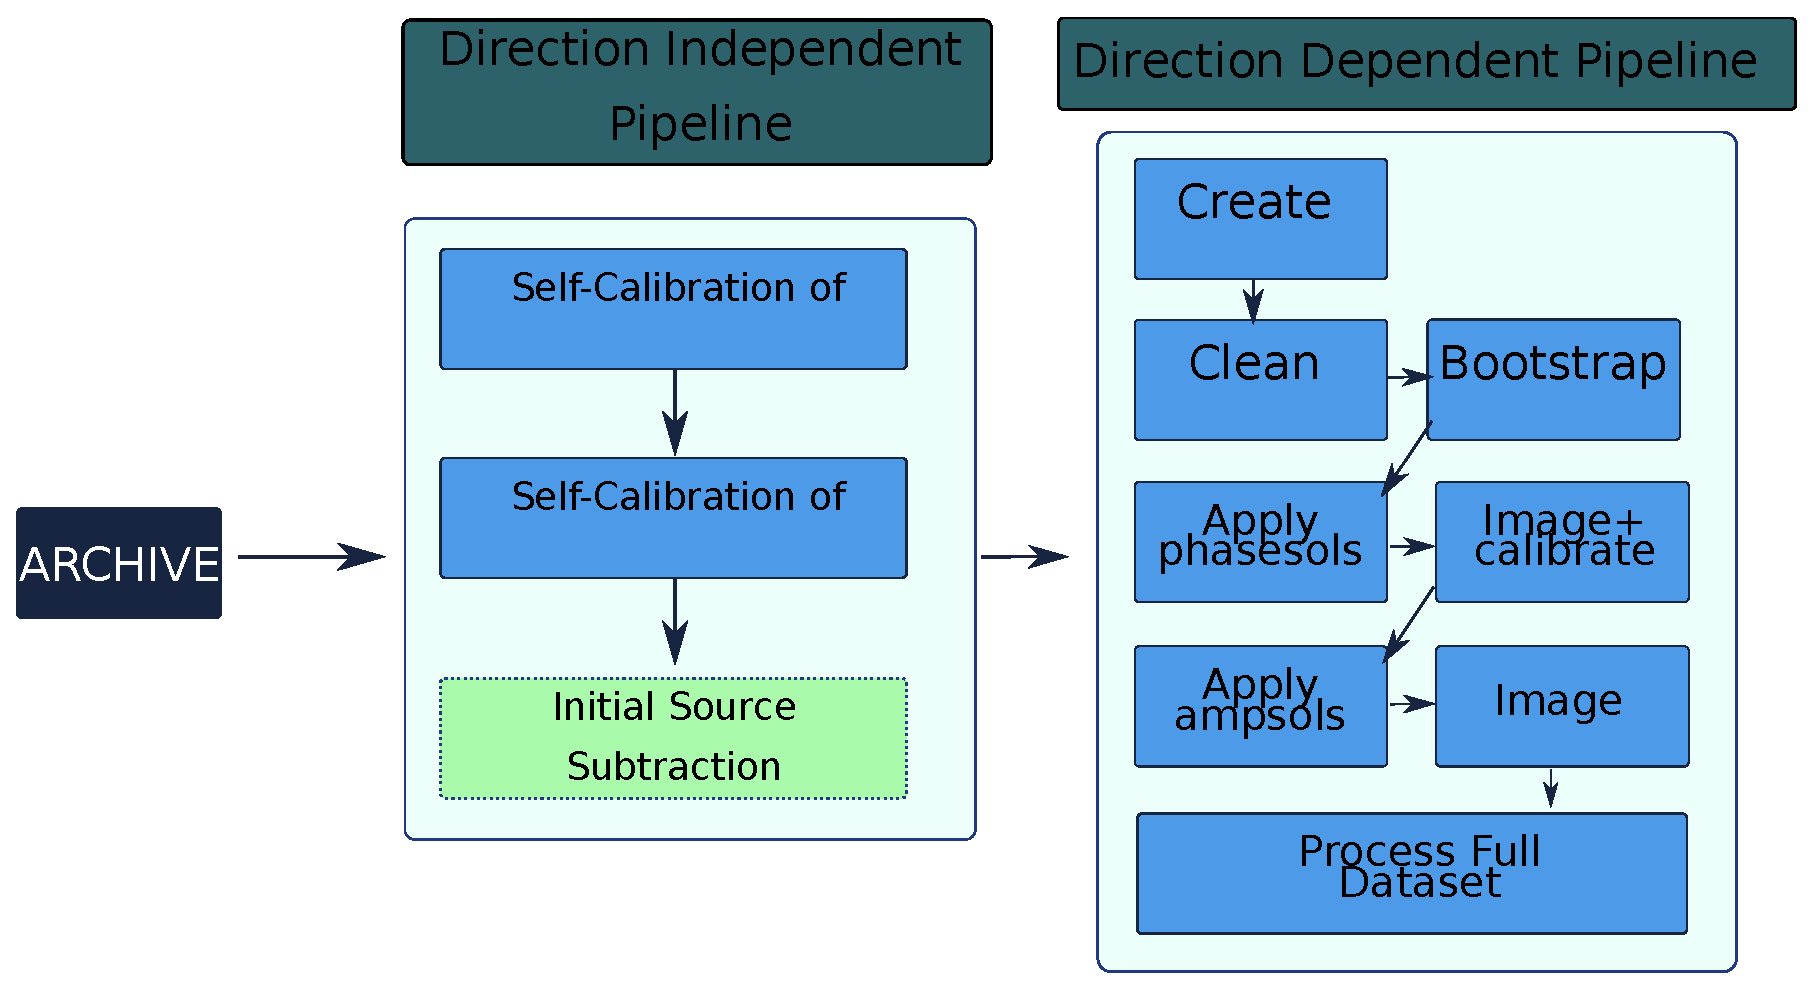
\includegraphics[width=.79\textwidth]{ch3/figures/DIDDpipe.eps}\\
 \caption[Prefactor and DDFacet Data Flow]{A schematic of the data flow through the Direction Independent Pipeline (pre-FACTOR\cite{prefactor}) and one of the Direction Dependent Pipelines (DDFacet). The Initial Source Subtraction is only necessary for some DD pipelines and is not currently implemented. }
 \label{fig:ch3_both_pipes}
\end{figure}


Data reduction for the LoTSS survey is split into two pipelines: Direction Independent (DI) calibration and Direction Dependent (DD) calibration (Fig\ref{fig:ch3_both_pipes}). The Direction Independent pipeline\cite{prefactor}\cite{van2016lofar} produces images that are limited in resolution and contain instrumental effects\cite{lotss}. To achieve high fidelity continuum images, the ionospheric and beam errors must be corrected\cite{lofar_calib}. As those effects vary across the field of view, a Direction Dependent calibration step must follow. Without these corrections the image quality and resolution is severely limited\cite{van2016lofar}.  We are currently working on a GRID implementation of the Direction Dependent pipeline and will report on this in a future paper.


\subsection{Direction Independent Processing}\label{sec:ch3_dirin_process}

The LOFAR telescope consists of many antennae, each with its own electronic gain. A gain calibration needs to be performed by observing a bright calibrator source before or after the science target\cite{lofar_calib}. Using this observation, the antenna gains for the telescope are calculated. This is performed by the Calibration pipeline of the pre-FACTOR software\cite{prefactor}.  The results from this step are applied to the science target and target observation is averaged  and processed. This consists of removing Radio Frequency Interference and subtraction of bright off-axis sources, and finally calibration against a sky model derived from surveys conducted with previous telescopes\cite{lofar_calib}\cite{van2016lofar}. These steps are performed by the Target pipeline of the pre-FACTOR software\cite{prefactor}. The result is a calibrated data set which is up to 64 times smaller than the uncalibrated archived data.

A 16TB data set cannot fit into a machine's memory, which is typically less than 128GB. Because of this,  the Direction Independent processing is be split by dividing the original full-bandwidth observation into independent chunks of narrower bandwidth. A typical observation spanning 48 MHz is split into 244 files called Subbands each of which spans 0.1953 MHz.  These Subbands are processed simultaneously, as each undergoes the same processing steps. This is a form of data-level parallelism. 

%The initial part of the LOFAR data processing can benefit from a cluster of many small machines. Doing so not only improves latency but allows for both scalability and fault tolerance, as discussed in Sections  \ref{sec:intermediate_storage} and \ref{sec:capabilities}. 

The Direction Independent calibration pipeline (Fig.\ref{fig:ch3_DIpipe}) consists of an existing set of scripts which use the LOFAR software suite\cite{lofarcookbook} to process the initial data sets. These scripts also handle the post-processing and application of the calibration results\cite{van2016lofar}. These scripts are contained in the package \emph{pre-FACTOR}\cite{prefactor}. The order of the scripts and their parameters are contained in a parameter-set file (henceforth 'parset'). The parset defines a sequence of procedures, each launching one or more executables. The execution of the procedures in a parset defines a step in the Direction Independent Pipeline. 


\subsection{Implementing the DI Calibration on the GRID}\label{sec:ch3_impl}

The LoTSS survey is mainly conducted by a team at Leiden University. The bandwidth between a University cluster and the LOFAR data archive is too low to download the data, 10 MB/s in the case of Leiden University. At Leiden University, downloading of one data set would take 10 times longer than the processing. The processing  was moved to the SURFsara grid location at the Amsterdam Science Park\footnote{http://docs.surfsaralabs.nl/projects/grid/en/latest/Pages/Service/system\_specs.html} as there were previous successes in processing LOFAR data at SURFsara (Oonk+ in prep).  In order to take advantage of the computational resources at the SURFsara Gina cluster\cite{gina_specs}, the LOFAR pre-FACTOR pipeline was modified as part of the development LRT framework. The two steps of the DI reduction, the Calibrator and Target, were each split in two parts. The first part of the Calibrator and Target processing is parallelized by running one file per node, and the second runs combine these results. This takes advantage of the data level parallelism of LOFAR processing.

Additionally, splitting the computation makes it more robust. In the case that the download or processing of one job fails, it can be restarted without disrupting parallel jobs. When a step has finished processing, the next step can be launched automatically enabling the massive processing of LOFAR Surveys data. 

The pre-FACTOR software was designed to be run on single machines or clusters with a shared file system. Because the worker machines at the SURFsara cluster have isolated storage, scripts are included in the LOFAR Reduction Tools to load the relevant data on the worker node before processing. After a job is finished, the scripts save intermediate results to a storage location external to the cluster. 

\subsection{Data Flow and Processing Steps}\label{sec:ch3_dataflow}

A researcher interested in processing LOFAR data needs to download it from the LOFAR Long Term Archive. Leiden University leads the LoTSS survey and has a computer cluster dedicated for LOFAR processing. The connection between the Leiden location and the LOFAR data archive is typically 10 MB/s. At this rate, downloading a single 16TB LoTSS data set completes in two weeks. At this rate, transferring 3000 data sets would take over a century. 

Unlike at Leiden University, the SURFsara clusters have a gigabit connection to the data archive, accelerating the data retrieval to 1.5 days. Additionally, having two orders of magnitude more processing nodes than at Leiden, the reduction can be further parallelized. This has accelerated the processing of one (downloaded) data set from more than two days to less than half a day.

Using intermediate storage to hold the results from each step, the pre-FACTOR DI pipeline (Fig.\ref{fig:ch3_both_pipes}) was split into four steps as in Fig. \ref{fig:ch3_DIpipe}. The Calib 1 and Target 1 steps download the raw data at one piece per worker machine and store the processing results (Calibration Tables and Processed data respectively) in storage. The second Calibration and Target steps combine these results and process them producing the calibration solutions and data sets respectively. 


\begin{figure}[H]
    \centering
 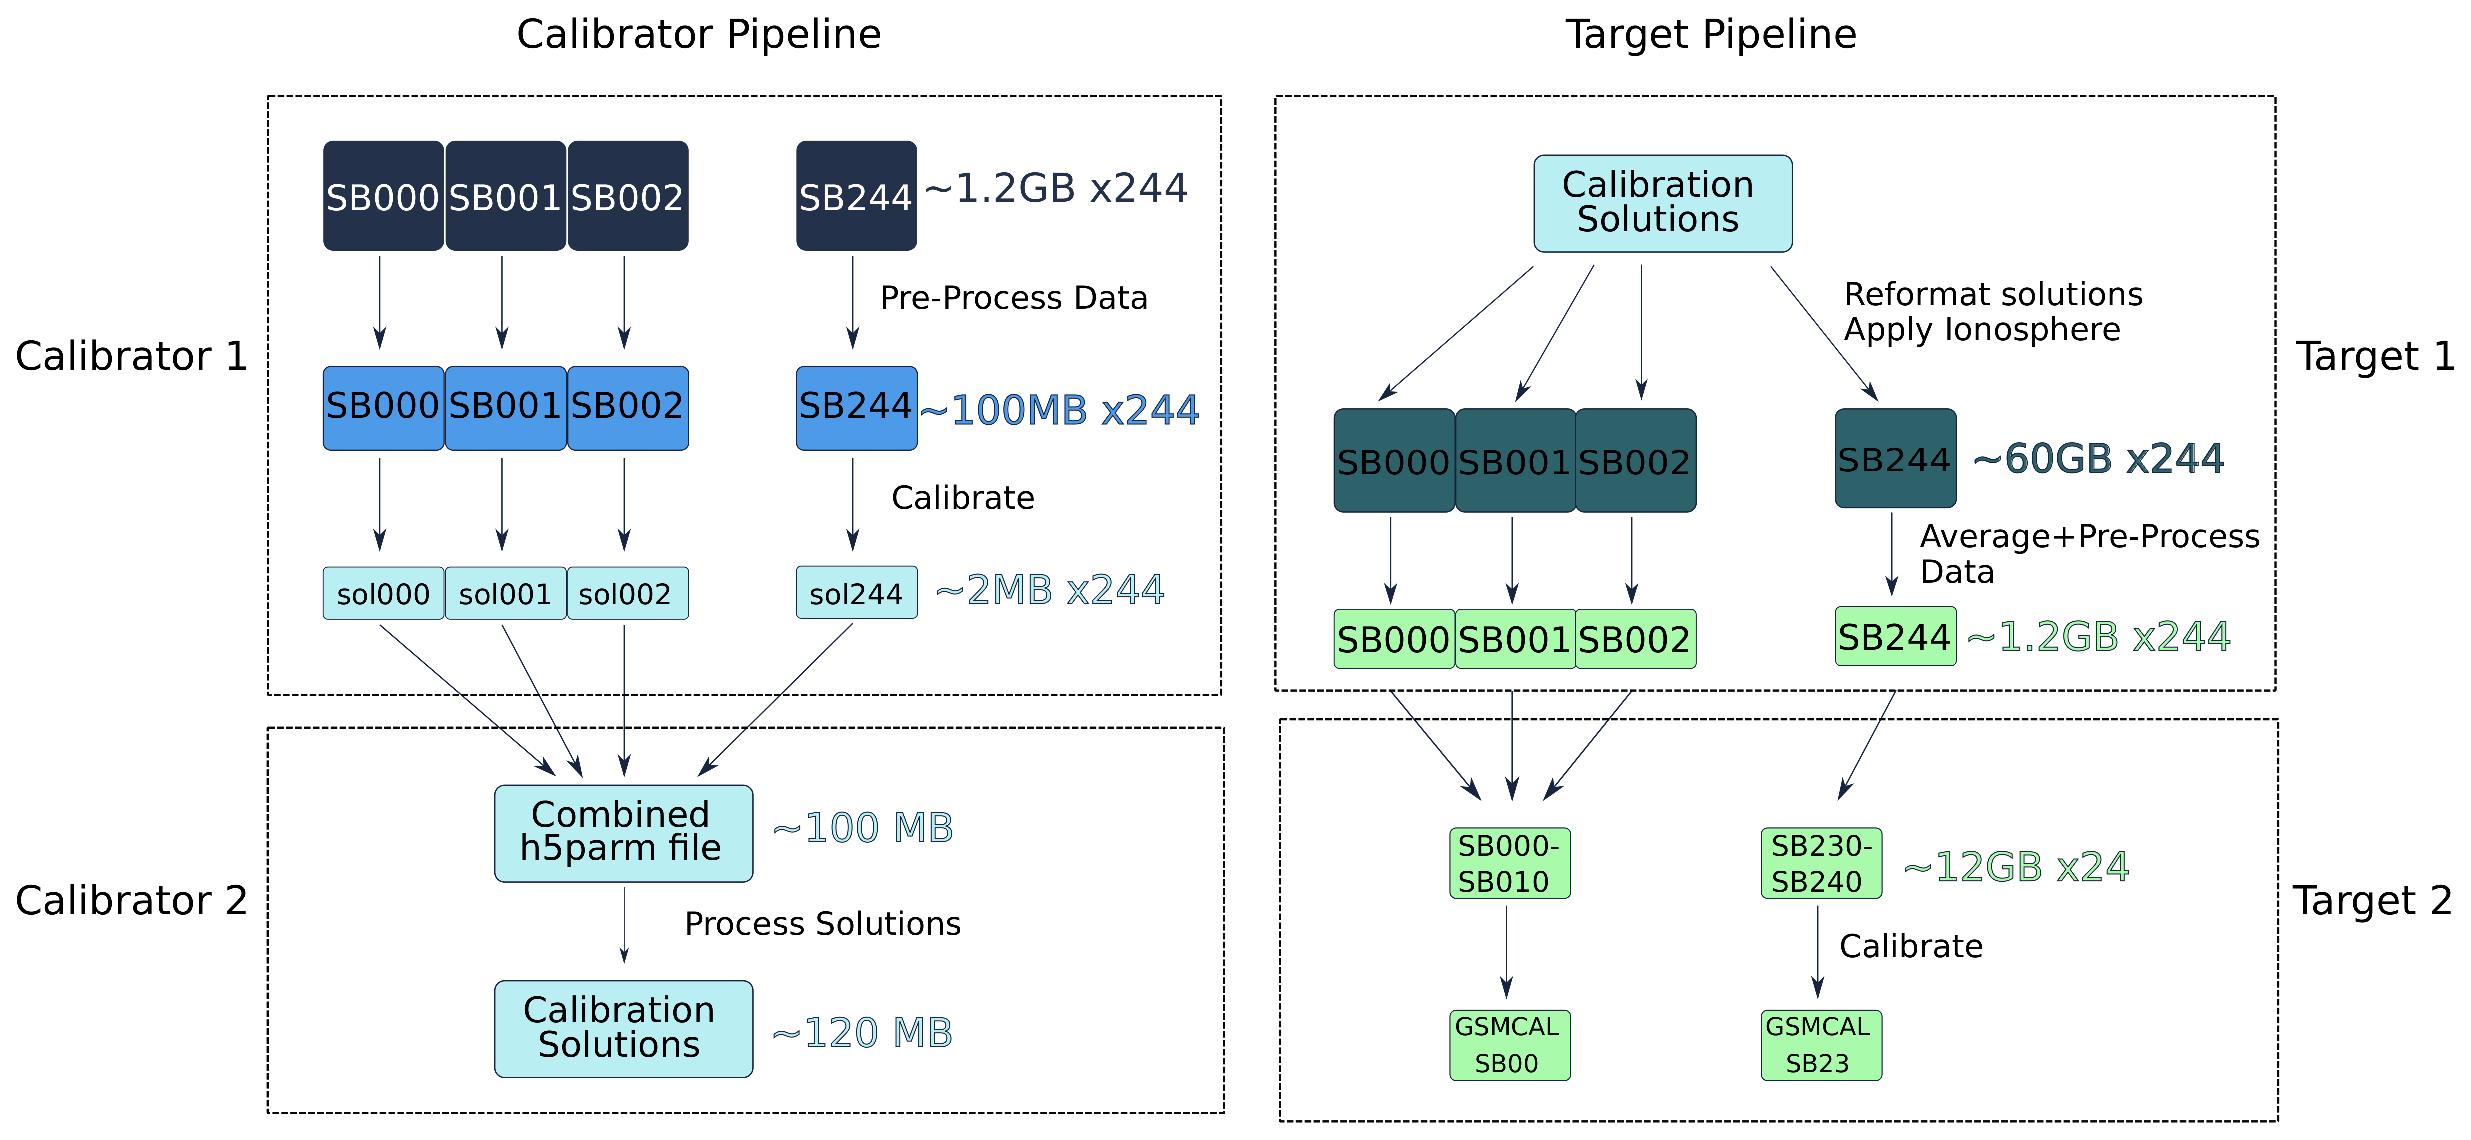
\includegraphics[width=.85\textwidth]{ch3/figures/Pipeline_parallel.eps}\\
    \caption[Parallelization of prefactor processing]{Data flow and parallelization of the Direction Independent Processing. The Calibrator 1 and Target 1 steps run concurrently as independent jobs. Calibrator 2 and Target 2 combine these results. Note that the Target 1 step requires the solutions produced by the Calibrator 2 step. This places a strict ordering on the processing steps. }
 \label{fig:ch3_DIpipe}
\end{figure}



\section{Framework Design}\label{sec:ch3_design}

The LRT framework (Fig. \ref{fig:ch3_design}) was developed to automate the LOFAR Direction Independent calibration by processing the data at the Gina cluster SURFsara\cite{gina_specs}. The goal of the framework was to adapt the pre-FACTOR package to take advantage of the large computational resources and high bandwidth at this site. Thanks to the data-level parallelism, using the computational resources at the Gina cluster accelerates the data reduction. 

\begin{figure}
 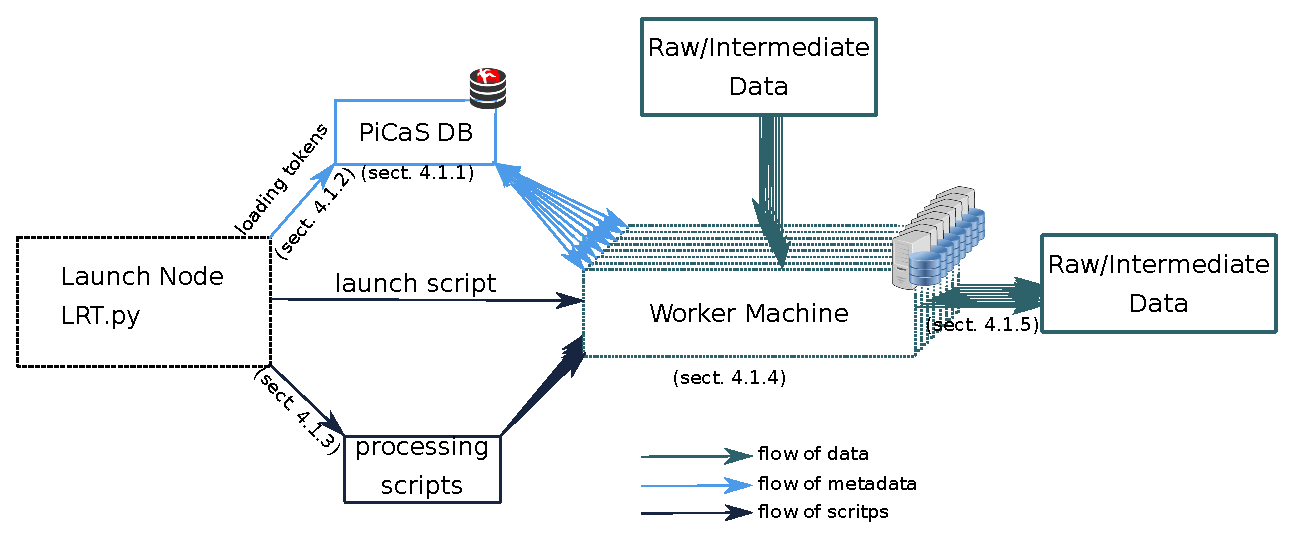
\includegraphics[width=0.7\textwidth]{ch3/figures/design.eps}\\
 \caption{Overview of the design of the LRT framework}
 \label{fig:ch3_design}
\end{figure}

\subsection{Framework Elements}
The LRT framework consists of a set of modules responsible for different parts of the data reduction. The \verb|srmlist| module handles the links to the data. If the data is on tape, it sends a command to stage it to disk. The \verb|sandbox| module creates an archive of processing scripts and uploads it to storage. The \verb|Token| module is responsible for managing metadata, which defines a processing job. Appendix \ref{sec:ch3_appendix_1} contains information on the functionality of each module and their use. 

\subsubsection{Storing Job Metadata}

The LRT framework is effective for pipelines that execute the same processing steps on a large data set split across many machines. Each part of the data set is processed on a single machine, and the metadata of this job is stored in a remote database which can be read from and written to by the worker machine. By using a concurrent document oriented database such as CouchDB\cite{couchdb}, each document can store the metadata regarding a single processing job. This is not possible with relational databases such as MySQL.  These documents are called Tokens, as defined by the PiCaS framework\cite{picas}.

The first implementation of PiCaS and CouchDB for LOFAR data reduction was carried by J. B. R. Oonk and N. Danezi in the context of the LOFAR spectroscopy project and custom user processing (Oonk et al. in prep). This first implementation focused on processing individual data sets and required a high-level of user interaction. Here we extend this implementation to automatically handle and connect multiple runs (calibrator and target) and their products.


By logging the name of the pipeline step in the job description, each job is aware of which pipeline step it is processing and executes the appropriate scripts. Important to note is that the CouchDB documents can store text and integer values as well as file attachments. The LOFAR implementation uses attachments to store diagnostic files produced by the worker machines, lists of links to the data and parset files that define the pre-FACTOR workflow. 

\subsubsection{Creating Job Tokens}\label{sec:ch3_create_tokens}

The first step to automating batch processing is to create the job tokens which hold the processing metadata and load them into the database. In order to track multiple concurrent reductions, these tokens are combined in sets. Once this set is given a name, a batch of tokens can be created for each pipeline step and uploaded into the PiCaS server. These tokens are set in the `todo' state, indicating the processing has not yet started. The specific implementation of the `pre-FACTOR' software is discussed in Appendix \ref{sec:ch3_appendix_1}.


\subsubsection{Packing Scripts}\label{sect:ch3_scripts}

While the PiCaS database can hold metadata which differs across jobs, pipelines or observations; the processing scripts need to be stored in a location where the worker machines have access to them. These scripts are archived and uploaded to storage and their location is added to the job token. After a worker machine locks a job token, it downloads and extracts the processing scripts, reads the metadata from the token and begins the processing (Fig.\ref{fig:ch3_tok_run}).

The location of the scripts is stored in the job token. This allows different steps of the pipeline to use different sets of scripts. The benefits from this design is that as long as the worker node has access to the URI (Universal Resource Identifier) of the scripts, it can process the data, making data reduction portable over a variety of distributed computing environments, including the GRID. This capability will be used in the future to move processing to the location of the archive (Section \ref{sec:ch3_future}). Implementation of this process is summarized in Appendix \ref{sec:ch3_appendix_1}. 


\subsubsection{Processing}

Processing is launched with a launch script executed on a worker node. This script is responsible for locking a job token, taking it from the `todo' state to the `locked' state. After the token is locked, the launch script downloads the script archive and launches the processing. For the LOFAR pre-FACTOR software, the scripts include the latest version of the pre-FACTOR repository. Additionally, there are helper scripts that set up the processing environment, download the data, post-process the output and upload the data to intermediate storage. The metadata stored in the PiCaS job token is fed into the setup and processing scripts. 

Since the processing scripts and metadata are stored remotely, the same small launch script can load many different reduction pipelines simply by changing the group of tokens it should lock.  This design choice makes it easy to create other script archives for the Direction Dependent pipeline or other LOFAR processing workflows. 

\begin{figure}
 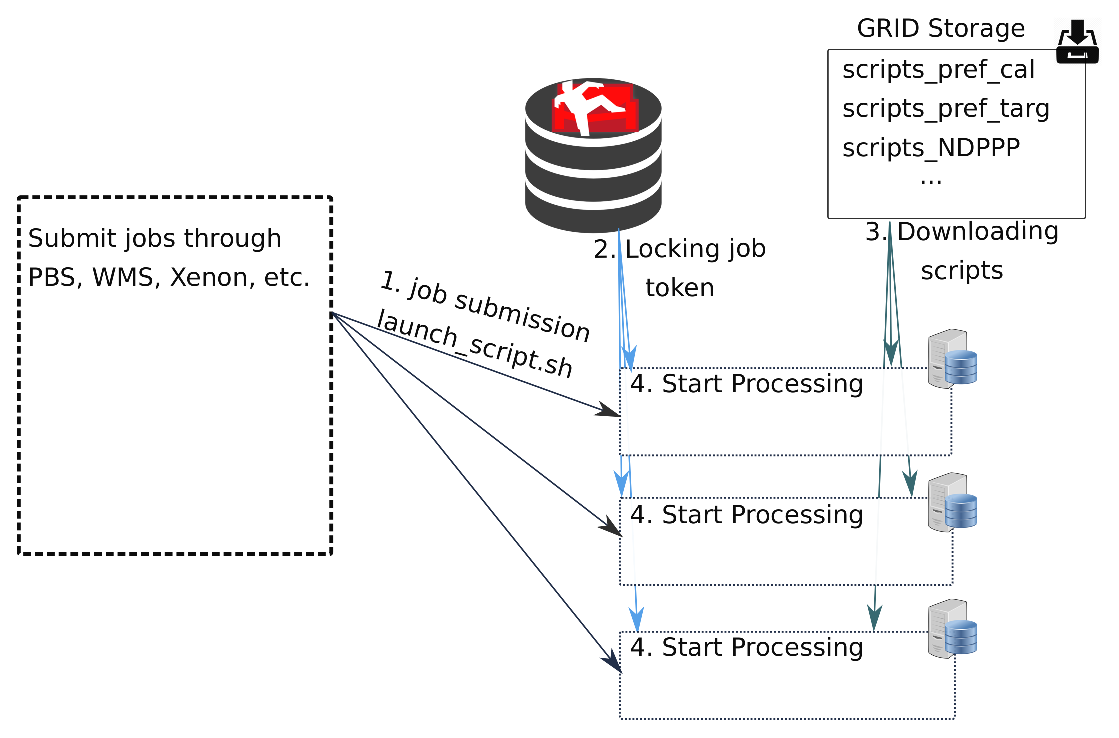
\includegraphics[width=.7\textwidth]{ch3/figures/token_run.eps}\\
    \caption[Starting processing on worker machines]{Starting processing on worker machines. Currently processing is done on SURFsara Gina nodes, however the framework has been tested at the Leiden University cluster.}
 \label{fig:ch3_tok_run}
\end{figure}


\subsubsection{Intermediate Data Storage}\label{sec:ch3_intermediate_storage}

Splitting the processing into multiple steps requires intermediate data to be stored at a location accessible to the worker machines. As the current processing is done at the Gina cluster, the intermediate results are stored in several dedicated
storage pools hosted by SURFsara. The LRT processing scripts check for the availability of an initial data set or intermediate data product on launch and download it. This avoids unnecessary repetition of reduction steps and allows to restarting a failed job.

Since the data location is static, the paths of the data are hard coded into the scripts. The framework design, however, also allows a job to log the location of its output data into the CouchDB database. Jobs in subsequent steps can read the location of their input data from the tokens of the previous job. This will be implemented when the LOFAR data processing becomes distributed across multiple locations. 

\begin{figure}
 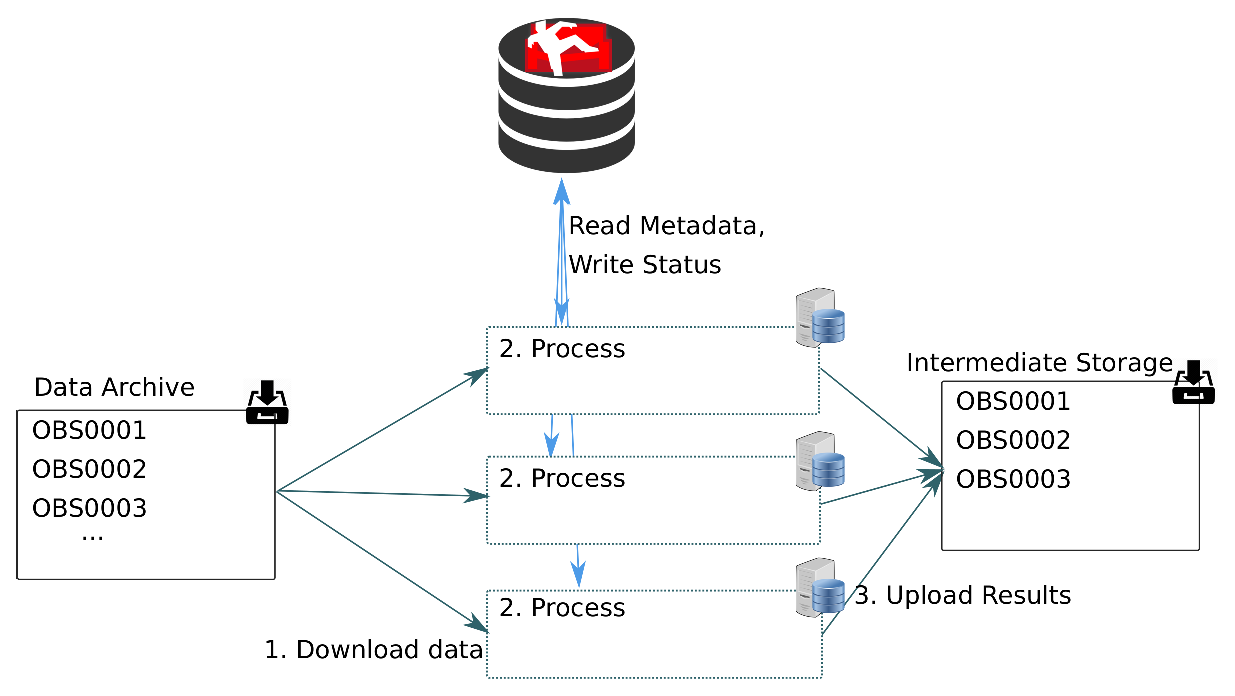
\includegraphics[width=.76\textwidth]{ch3/figures/token_process.eps}\\
    \caption[Schematic of data movement.]{Processing of LOFAR data from the Long Term Archive with results stored at an intermediate storage location.}
 \label{fig:ch3_tok_process}
\end{figure}

\subsection{LOFAR Surveys Use Case}\label{sec:ch3_use}
The LOFAR Two Meters Sky Survey requires processing of more than 8 PB of data each year in order to keep up with the data produced by the telescope. As there are more than 3000 observations planned, processing them manually is untenable. Additionally, the large raw data sizes require the data be reduced in parallel before the Direction Dependent calibration step since the data will not fit in the memory of a single machine. 

Re-purposing the LOFAR pre-FACTOR software to take advantage of the GRID computing resources by leveraging the automation provided by the LRT framework has allowed the processing of more than a hundred data sets in the time span of four months. Additionally, this was done in the time frame that an astronomer would normally produce less than 10 Direction Independent calibrated observations, hence a providing a necessary speed up by an order of magnitude.


\subsection{Framework Capabilities}\label{sec:ch3_capabilities}

The LRT implementation is designed to be as platform independent as possible. It allows for easy extensions enabling LOFAR reduction schemes other than the LoTSS reduction. Two examples of this are the updated LOFAR GRID spectroscopy and LOFAR GRID pre-processing pipelines (Oonk+ in prep). The GRID pre-processing pipeline runs flagging of bad data and averaging, however performs no calibration. The spectroscopy pipeline uses an independent set of scripts to perform calibration,  bandwidth correction and imaging. 

Thanks to the abstraction of the metadata and scripts storage, processing is also possible at other locations. The pre-FACTOR scripts require an installation of the LOFAR software stack\cite{lofar_stack}. These requirements are met by mounting a CernVM-FS\cite{cvmfs2008}\cite{softdrive} installation of the LOFAR stack. The CERN-VM FileSystem service provides a portable pre-compiled copy of the LOFAR software.  With the CVMFS prerequisite satisfied and an active grid proxy, any computer can download data and process a job in any data reduction step. 


\subsection{Initial Results}\label{sec:ch3_performance_results}

Automatically launching jobs has made it possible to process more than 100 data sets between November 2016 and February 2017. Without a framework to automate and distribute the processing and a cluster at a Grid location, these data sets would need to be downloaded to an institute's cluster. Such standalone runs of the `pre-FACTOR' scripts typically process one observation in two weeks taking into account the data transfer time.  At the 10MB/s connection (The sustained speed at Leiden University), the downloading would take over 5 years alone. Porting the LOFAR LoTSS data reduction to a Grid location using the LRT framework has resulted in a 15x increase in data throughput. Suggestions on further increasing the throughput are presented in Section \ref{sec:ch3_future}.
 
% \subsection{Bottlenecks and Proposed Solutions}
% 
% Launching multiple processing jobs leads to large data transfer rates between the raw data archive and the processing site. While the SURFsara Grid location has a gigabit connection to the data archives, launching more than two reductions at a time results in a download bottleneck. This bottleneck is caused by the 1 Gbps public connection between LTA sites. Most of the LoTSS data is stored at the Forschungszentrum Jülich location. Thus, the 1Gbps bandwidth between the archive and processing sites limits the download to 35 hours per 16TB observation. To process the outstanding data within the five project time line, the minimum bandwidth requirement is a 2.5 Gbps uninterrupted connection to the data. Solutions to this bottleneck are presented in Section \ref{sec:future}. 


\section{Conclusion and Future Work}\label{sec:ch3_conclusion}

The goal of the LRT Framework is to create an automated software which can be used to port LOFAR processing to a massively distributed compute environment. The Direction Independent calibration of the LOFAR Two Meter Sky Survey was used as a demonstration of the capabilities of the LRT software. 

Combining the `pre-FACTOR' scripts with the LRT tools resulted in a 15x increase in throughput compared to previous data reduction strategies. Thanks to the automation provided, it is possible to process hundreds of observations, necessary for large astronomical survey projects such as the 3000+ observations of the LoTSS. 

The scalability of this framework allows to launch multiple data reductions concurrently and easily monitor their progress. The portability of the LRT framework makes it easy to move processing to archive locations, further increasing the throughput. Finally, as the framework is general, other LOFAR projects can increase throughput and automation by integrating their software. 


\subsection{Throughput Improvement}

Using the LRT framework, more than 100 data sets have passed through the Direction Independent calibration. This is more than a 15 fold increase compared to the throughput at a institution with a limited bandwidth to the data archive. From these data sets, 30 images have been produced since November 2016.  The Direction Dependent pipeline, responsible for the imaging of the DI calibrated data, is not yet automated using the LRT framework. The topic of this automation will be handled in future work. Future improvements (Section \ref{sec:ch3_future}) are expected to increase the throughput to one image per day.  

Currently, the data reduction is launched manually. There are upcoming plans to create a trigger launched by the Observatory at the end of a successful observation. Using this trigger, the processing can be integrated with the data acquisition and launched automatically at the end of the observation. Doing so enables producing an image less than a week after the observation has completed without requiring human interaction. 
% 
\subsection{Future Work}\label{sec:ch3_future}


Most of the LoTSS data is not stored at the SURFsara Grid location. Because of the high data sizes, the 1 Gbps transfer between these remote sites and SURFsara is insufficient to process the 3000+ data sets. The proposed solution is to launch the initial reduction steps (Calibrator 1 and Target 1 in Fig.\ref{fig:ch3_DIpipe}) on compute clusters at the archive locations. Running the Target 1 step at these sites will reduce the data size from 16TB to 0.5TB. The resulting intermediate data can easily be transferred over a 1 Gbps connection in 1 hour compared with the 35 hours for the original data. 

While the LRT framework successfully automated the Direction Independent calibration pipeline, it still needs to  implement the Direction Dependent processing scripts. The DI data can be easily split into pieces and processed concurrently, however current Direction Dependent pipelines cannot split the data easily. This means they will only benefit from the automation aspect of the framework. Because of this limitation of the algorithms, (Direction Dependent) processing of each data set needs to be done on a single machine.  This part of the processing currently takes more than four days per data set per node. To process all 3000 observations within five years, the DD reduction will need at least 8 dedicated machines continuously processing data. Nevertheless, the input data is only 200-500GB making it easier to store and transfer to institutes not part of the European Grid Infrastructure. 

The Xenon framework\cite{maasen_xenon} allows launching jobs at multiple clusters from a single location. Thanks to the portability of the LRT software, it will be possible to integrate the LOFAR reduction with Xenon. This will automate the launching of Direction Dependent processing at multiple institutions. Automatically launching these jobs will make efficient use of the computer resources at SURFsara and other sites. Using this strategy, the LoTSS project data can be processed within the anticipated time span. 

Finally, as the reduction is automated, it can be started right after the telescope finishes the observation. Launching jobs immediately after  an observation will minimize the time staging the data from tape to disk. Currently, the staging process can take up to a week. Triggering the processing immediately after observation, an image will be produced less than a week after the data is acquired. 

Minimizing the latency between observation and science quality images will benefit the LOFAR community immensely by allowing radio astronomers to focus on their specific science case. An all-sky survey at the 150 MHz range will create a multitude of targets for follow-up with optical telescopes and result in many discoveries in the field of Radio Astronomy. A full list of science results expected from the LoTSS project can be found in\cite{lotss}. Efficient high-throughput processing of LOFAR data will empower the above science cases opening the way to  exciting new discoveries.


\begin{subappendices}

\section{Execution of LOFAR Reduction Tools }\label{sec:ch3_appendix_1}

The LRT framework handles staging of LOFAR data, packaging and uploading worker node scripts (named sandboxes), creating PiCaS job tokens and launching pilot jobs on the SURFsara Gina cluster. The framework is modular, allowing an user to execute any of the previous steps manually, or alternatively launch an automated reduction. It can be downloaded from the Github page (\href{https://github.com/apmechev/GRID_LRT}{github.com/apmechev/GRID\_LRT}) and installed with \\
\verb|python setup.py build && python setup.py install| . Documentation on the usage of the tools can be found at the Github page. 
\end{subappendices}


% \begin{thebibliography}{99}
%\bibitem{softdrive}
%Softdrive on the grid.
%\newblock Available at
%  \url{http://docs.surfsaralabs.nl/projects/grid/en/latest/Pages/Advanced/grid\_software.html\#softdrive
%  }.
%
%\bibitem{gina_specs}
%Gina specifications - grid documentation v1.0.
%\newblock Available at
%  \url{http://docs.surfsaralabs.nl/projects/grid/en/latest/Pages/Service/system\_specifications/gina\_specs.html},
%  2017.
%
%\bibitem{lofar_stack}
%Lofar software stack.
%\newblock
%  \url{http://www.lofar.org/wiki/doku.php?id=public:software\_stack\_installation},
%  2017.
%
%\bibitem{picas}
%Picas overview - grid documentation v1.0.
%\newblock
%  \url{http://doc.grid.surfsara.nl/en/latest/Pages/Practices/picas/picas\_overview.html},
%  2017.
%
%\bibitem{prefactor}
%Horneffer A.
%\newblock Prefactor: Pre-facet calibration pipeline.
%\newblock \url{https://github.com/lofar-astron/prefactor}, 2017.
%
%\bibitem{cvmfs2008}
%C~Aguado~Sanchez, J~Bloomer, P~Buncic, L~Franco, S~Klemer, and P~Mato.
%\newblock Cvmfs-a file system for the cernvm virtual appliance.
%\newblock In {\em Proceedings of XII Advanced Computing and Analysis Techniques
%  in Physics Research}, volume~1, page~52, 2008.
%
%\bibitem{couchdb}
%Chirs ANDERSON.
%\newblock Apache couchdb: The definitive guide.
%\newblock {\em http://couchdb. Apache. org/index. htm Acessado em}, 5(06):2009,
%  2009.
%
%\bibitem{ska_cloud_memo}
%Domingos Barbosa, Jo{\~a}o~Paulo Barraca, Dalmiro Maia, Bruno Carvalho, Jorge
%  Vieira, Paul Swart, Gerhard Le~Roux, Swaminathan Natarajan, Arnold van
%  Ardenne, and Luis Seca.
%\newblock Power monitoring and control for large scale projects: Ska, a case
%  study.
%\newblock In {\em SPIE Astronomical Telescopes+ Instrumentation}, pages
%  99100L--99100L. International Society for Optics and Photonics, 2016.
%
%\bibitem{simcity}
%Joris Borgdorff, Harsha Krishna, and Michael~H Lees.
%\newblock Sim-city: An e-science framework for urban assisted decision support.
%\newblock {\em Procedia Computer Science}, 51:2327--2336, 2015.
%
%\bibitem{picas_git}
%Jan Bot.
%\newblock Picas: Python client using couchdb as a token pool server.
%\newblock \url{https://github.com/jjbot/picasclient}, 2017.
%
%\bibitem{clemencic2014new}
%Marco Clemencic and B~Couturier.
%\newblock A new nightly build system for lhcb.
%\newblock In {\em Journal of Physics: Conference Series}, volume 513, page
%  052007. IOP Publishing, 2014.
%
%\bibitem{lofar_data}
%Hanno Holties, Adriaan Renting, and Yan Grange.
%\newblock The lofar long-term archive: e-infrastructure on petabyte scale.
%\newblock In {\em SPIE Astronomical Telescopes+ Instrumentation}, pages
%  845117--845117. International Society for Optics and Photonics, 2012.
%
%\bibitem{cvmfsatlas}
%Grigory Rybkin.
%\newblock Atlas software packaging.
%\newblock In {\em Journal of Physics: Conference Series}, volume 396, page
%  052063. IOP Publishing, 2012.
%
%\bibitem{li2017reliability}
%Y~Li.
%\newblock Reliability of long heterogeneous slopes in 3d: Model performance and
%  conditional simulation.
%\newblock 2017.
%
%\bibitem{maasen_xenon}
%Jason Maassen, Stefan Verhoeven, Joris Borgdorff, Niels Drost, cwmeijer,
%  Jurriaan~H. Spaaks, Rob~V. van Nieuwpoort, Piter~T. de~Boer, and Ben van
%  Werkhoven.
%\newblock Xenon: Xenon 1.1.0, December 2015.
%
%\bibitem{lofarcookbook}
%RF~Pizzo et~al.
%\newblock The lofar imaging cookbook v2.0.
%\newblock {\em internal ASTRON report}, 2010.
%
%\bibitem{sante2010development}
%Tom SANTE.
%\newblock Development of (graphical) web applications for the processing and
%  interpretation of arraycgh data.
%\newblock 2010.
%
%\bibitem{lotss}
%TW~Shimwell, HJA R{\"o}ttgering, PN~Best, WL~Williams, TJ~Dijkema,
%  F~de~Gasperin, and MJ~Hardcastle.
%\newblock The lofar two-metre sky survey. i. survey description and preliminary
%  data relase.
%\newblock {\em Astronomy \& Astrophysics}, 2016.
%
%\bibitem{lofar_calib}
%Cyril Tasse, Ger van Diepen, Sebastiaan van~der Tol, Reinout~J van Weeren,
%  Joris~E van Zwieten, Fabien Batejat, Sanjay Bhatnagar, Ilse van Bemmel, Laura
%  B{\^\i}rzan, Annalisa Bonafede, et~al.
%\newblock Lofar calibration and wide-field imaging.
%\newblock {\em Comptes Rendus Physique}, 13(1):28--32, 2012.
%
%\bibitem{van2013lofar}
%MP~Van~Haarlem, MW~Wise, AW~Gunst, George Heald, JP~McKean, JWT Hessels,
%  AG~De~Bruyn, Ronald Nijboer, John Swinbank, Richard Fallows, et~al.
%\newblock Lofar: The low-frequency array.
%\newblock {\em Astronomy \& Astrophysics}, 556:A2, 2013.
%
%\bibitem{van2016lofar}
%RJ~Van~Weeren, WL~Williams, MJ~Hardcastle, TW~Shimwell, DA~Rafferty, J~Sabater,
%  G~Heald, SS~Sridhar, TJ~Dijkema, G~Brunetti, et~al.
%\newblock Lofar facet calibration.
%\newblock {\em The Astrophysical Journal Supplement Series}, 223(1):2, 2016.
%
%\bibitem{bioinfo}
%Anjani Ragothaman, Sairam~Chowdary Boddu, Nayong Kim, Wei Feinstein, Michal
%  Brylinski, Shantenu Jha, and Joohyun Kim.
%\newblock Developing ethread pipeline using saga-pilot abstraction for
%  large-scale structural bioinformatics.
%\newblock {\em BioMed research international}, 2014, 2014.
%
%\bibitem{ecoinfo}
%William~K Michener and Matthew~B Jones.
%\newblock Ecoinformatics: supporting ecology as a data-intensive science.
%\newblock {\em Trends in ecology \& evolution}, 27(2):85--93, 2012.
%
%\bibitem{swift}
%Yong Zhao, Mihael Hategan, Ben Clifford, Ian Foster, Gregor Von~Laszewski,
%  Veronika Nefedova, Ioan Raicu, Tiberiu Stef-Praun, and Michael Wilde.
%\newblock Swift: Fast, reliable, loosely coupled parallel computation.
%\newblock In {\em Services, 2007 IEEE Congress on}, pages 199--206. IEEE, 2007.
%
%\bibitem{scalable}
%Shayan Shams, Nayong Kim, Xiandong Meng, Ming~Tai Ha, Shantenu Jha, Zhong Wang,
%  and Joohyun Kim.
%\newblock A scalable pipeline for transcriptome profiling tasks with on-demand
%  computing clouds.
%\newblock In {\em Parallel and Distributed Processing Symposium Workshops, 2016
%  IEEE International}, pages 443--452. IEEE, 2016.
%
%\bibitem{aperturesynth}
%WN~Brouw.
%\newblock Aperture synthesis.
%\newblock In {\em Image Processing Techniques in Astronomy}, pages 301--307.
%  Springer, 1975.
%
%\bibitem{neurogrid}
%JD~Van~Horn, J~Dobson, J~Woodward, M~Wilde, Y~Zhao, J~Voeckler, and I~Foster.
%\newblock Grid-based computing and the future of neuroscience computation,
%  methods in mind, 2005.
%  
%\bibitem{cvmfsnova}
%GS~Davies, JP~Davies, Brian Rebel, Kanika Sachdev, Jan Zirnstein, C~Group,
%  et~al.
%\newblock Software management for the no$\nu$aexperiment.
%\newblock In {\em Journal of Physics: Conference Series}, volume 664, page
%  062011. IOP Publishing, 2015.
%
%\bibitem{pegasus}
%Ewa Deelman, Gurmeet Singh, Mei-Hui Su, James Blythe, Yolanda Gil, Carl
%  Kesselman, Gaurang Mehta, Karan Vahi, G~Bruce Berriman, John Good, et~al.
%\newblock Pegasus: A framework for mapping complex scientific workflows onto
%  distributed systems.
%\newblock {\em Scientific Programming}, 13(3):219--237, 2005.
%
%\end{thebibliography}
%
% \end{document}
